\begin{figure*}[!t]
  \setlength{\abovecaptionskip}{4pt}
  \centering
  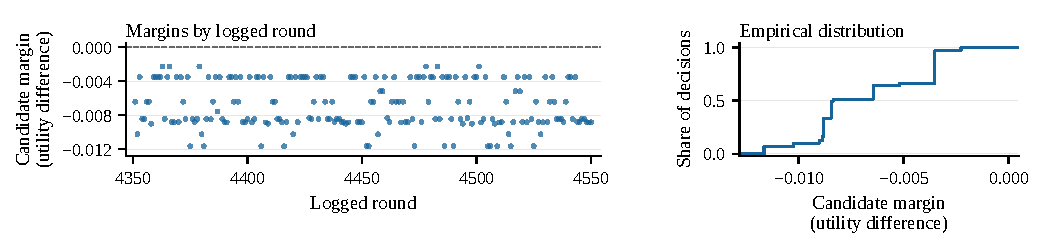
\includegraphics[width=\linewidth]{figures/fig_candidate_margin_window.pdf}
  \caption{\textbf{Adapter candidates remain below prior retained utility in the fixed window.}
  All 200 recorded admission decisions in rounds 4351--4550, captured at
  23:20 UTC on 3 November 2026. Left: candidate utility minus the explicit
  pre-decision retained utility; negative values mean lower candidate utility.
  Right: the empirical cumulative distribution of the same 200 signed margins,
  weighting each decision equally. The journal records zero admissions.
  No smoothing, imputation or cumulative minimum is applied.
  These adaptive development-pool observations do not establish an independent
  learning gain. Scope: \cref{sec:method-status}.}
  \label{fig:candidate-margin-window}
\end{figure*}

\subsection{A later candidate-margin window}\label{app:candidate-margin-window}

\Cref{fig:candidate-margin-window} follows the earlier pre-decision margin
view in \cref{fig:fw-admission-margins} with a fixed later window.
Its empirical distribution counts decisions, not independent tasks or
programs; the common telemetry scope applies (\cref{sec:method-status}).
